\documentclass[15pt,a4paper]{article}

%use the english line for english reports
%usepackage[english]{babel}
\usepackage[portuguese]{babel}
\usepackage[utf8]{inputenc}
\usepackage{indentfirst}
\usepackage{graphicx}
\usepackage{moreverb}
\usepackage{subfig}
\usepackage{float}
\usepackage{url}

\floatstyle{ruled}
\newfloat{code}{!ht}{lop}
\floatname{code}{Código fonte}


\begin{document}

\setlength{\textwidth}{16cm}
\setlength{\textheight}{22cm}


%************************************************************************************************
%************************************************************************************************

\title{
	\Huge\textbf{Breakthrough}
	\linebreak\linebreak\linebreak
	\Large\textbf{Relatório}
	\linebreak\linebreak
	
\includegraphics[height=6cm, width=7cm]{feup.pdf}
	\linebreak \linebreak
	\Large{Mestrado Integrado em Engenharia Informática e Computação}
	\linebreak\linebreak
	\Large{Programação em Lógica}\linebreak
}


\author{\textbf{Grupo 17:}
\\ João Guedes - 070509043
\\ João Henriques - 110509026
\\\linebreak\linebreak \\
\\ Faculdade de Engenharia da Universidade do Porto
\\ Rua Roberto Frias, s\/n, 4200-465 Porto, Portugal
\linebreak\linebreak\linebreak
\linebreak\linebreak\vspace{1cm}}
\date{Setembro de 2011}
\maketitle
\thispagestyle{empty}



%************************************************************************************************
%************************************************************************************************


\section*{Resumo}

% Descrever muito sumariamente o trabalho. Deve ser suficiente para o leitor decidir se lê ou não o resto do relatório.
% Não deve incluir nenhuma referência ao facto de ser feito no âmbito de uma cadeira.



O \textit{Breakthrough} é um jogo de tabuleiro tradicional semelhante às damas, premiado e com um conjunto de regras muito simples e acessíveis.

A implementação ferece dois modos de jogo - Humano/Humano e Humano/Computador.

A linguagem utilizada para esta implementação foi \textit{ProLog}.

\tableofcontents

%************************************************************************************************
%************************************************************************************************

\newpage


\section{Introdução}

% Descrever os objectivos e motivação do trabalho. Não deve incluir nenhuma referência ao facto de ser feito no âmbito de uma cadeira.
% Último parágrafo deve indicar a estrutura do relatório.
% Devem ser incluídas referências bibliográficas correctas e completas (consultar os docentes em caso de dúvida). Páginas da wikipedia não são consideradas referências válidas \cite{CodigoSite, %CodigoLivro}.
% Todas as figuras devem ser referidas no texto. %\ref{fig:codigoFigura}



Este trabalho tem como principal motivação a consolidação do nosso conhecimento em ProLog, visto que o paradigma de programação é totalmente diferente daquele a que temos vindo a estar habituados ao longo do curso.

Por ser menos exigente e mais exequível dados os nossos conhecimentos, começaremos por implementar o modo Humano/Humano através de regras lógicas.

Seguidamente recorreremos a algoritmos de inteligência artificial e à teoria dos jogos para implementar os modos que envolvam o Computador.


Escolhemos este trabalho porque gostamos da sua simplicidade e fluidez, e apesar de não ter um conjunto de regras muito vasto, é um jogo com potencial estratégico. 
Se o oponente não estiver atento é capaz de ser vencido muito rapidamente.

De notar que, apesar da nossa implementação consistir num tabuleiro convencional de 8x8, o \textit{Breakthrough} pode ser jogado com outras configurações, como tabuleiros 7x7 ou tabuleiros não-quadrados.

%************************************************************************************************
%************************************************************************************************

\section{Descrição do Problema}

%Descrever sucintamente o jogo, a sua história e, principalmente, as suas regras. Devem ser criadas/utilizadas imagens apropriadas para explicar o funcionamento do jogo.

O \textit{Breakthrough} foi criado no ano 2000 por \textit{Dan Troyka}  e disponibilizado para a plataforma comercial \textit{Zillion of Games}.

\subsection{Preparação de jogo}
\begin{enumerate}
\item Cada jogador começa com 16 peças uniformes, distribuidas pelas duas linhas mais próximas de si, à semelhança dum tabuleiro de xadrez.
\item Os dois jogadores escolhem o seu lado e é sorteado o primeiro a começar.
\end{enumerate}

\subsection{Movimentos permitidos}
\begin{enumerate}
\item Um jogador pode mover uma peça se a casa de destino estiver vazia, diagonalmente ou em frente, conforme ilustrado.
\item Os jogadores movimentam-se sempre em direção à base do adversário, e nunca podem retroceder.
\item Quando o jogador avança em direção à base oposta e se depara com uma peça adversária diagonalmente, pode capturá-la, sendo a peça capturada eliminada do tabuleiro e substituída pela peça do capturador. 
No entanto a captura não é obrigatória nem encadeada como nas damas.
\end{enumerate}

%Figura 1
\begin{figure}[h!]
\begin{center}
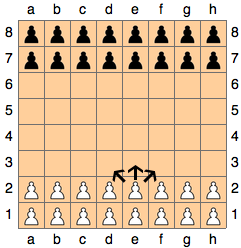
\includegraphics[scale=0.5]{fig1.png}
\caption{Movimento possível da peça e2}
\label{fig:1}
\end{center}
\end{figure}

%Figura 2 (a e b)
\begin{figure}[H]
\begin{center}
\subfloat[Possibilidades para a peça f3]{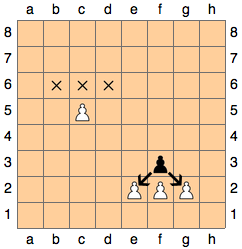
\includegraphics[scale=0.5]{fig2a.png}\label{fig:2a}}\hspace{10px}
\subfloat[Captura de e2]{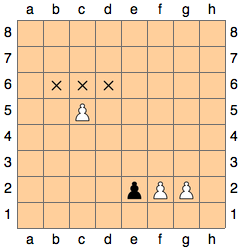
\includegraphics[scale=0.5]{fig2b.png}\label{fig:2b}}
\caption{Processo de captura.}
\label{fig:2}
\end{center}
\end{figure}

\subsection{Vitória}
\begin{enumerate}
\item O primeiro jogador a atingir a base do adversário, vence. No caso anterior, se o jogador 2 (peças pretas) atingisse a linha 1, venceria.
\item Se todas as peças de um jogador forem capturadas, este perde o jogo.
\item Um empate é matemáticamente impossível, e todas as peças têm sempre pelo menos uma jogada na diagonal possível.
\end{enumerate}


%************************************************************************************************
%************************************************************************************************
\newpage

\section{Arquitectura do Sistema}
Descrever em linhas gerais o sistema e os módulos que o constituem. Deve ser abordada a comunicação com o visualizador, que mesmo que ainda não esteja implementada, já deverá estar pensada. Assim, deve ser incluída a sintaxe das mensagens a trocar com o visualizador.


%************************************************************************************************
%************************************************************************************************
\newpage

\section{Módulo de Lógica do Jogo}
Descrever o projecto e implementação do módulo Prolog, incluindo a forma de representação do estado do tabuleiro,  verificação do cumprimento das regras do jogo, determinação do final do jogo e cálculo das jogadas a realizar pelo computador  utilizando diversos níveis de jogo.

%************************************************************************************************

\subsection{Representação do Estado do Jogo} \textit{estado(?Tabuleiro).}

%************************************************************************************************
\subsection{Visualização do Estado do Jogo} \textit{visualiza\_estado(+Tabuleiro).}

%************************************************************************************************
\subsection{Validação de Jogadas} \textit{movimento\_valido(?Jogada, +Tabuleiro).}

%************************************************************************************************
\subsection{Execução de Jogadas}\textit{executa\_movimento(+Jogada, + Tabuleiro, -NovoTabuleiro).}

%************************************************************************************************
\subsection{Lista de Jogadas Válidas}\textit{lista\_jogadas(+Tabuleiro, -ListaJogadas).}

%************************************************************************************************
\subsection{Avaliação do Tabuleiro}\textit{avalia\_tabuleiro(+Tabuleiro, -Valor).}

%************************************************************************************************
\subsection{Final do Jogo} \textit{fim\_jogo(+Tabuleiro, -Vencedor).}

%************************************************************************************************
\subsection{Cálculo da Jogada do Computador}\textit{calcula\_jogada(+Nível, +Tabuleiro, -Jogada).}

%************************************************************************************************
\subsection{Recepção de mensagem do visualizador}\textit{recebe\_mensagem(+ Mensagem, - Resposta).}


%************************************************************************************************
%************************************************************************************************
\newpage

\section{Conclusões e Perspectivas de Desenvolvimento}

% Que conclui da análise do jogo e da pesquisa bibliográfica realizada?
% Como vai ser desenvolvido o trabalho?
% Que parte (\%) do trabalho estima que falta fazer?

Dados os conhecimentos adquiridos, podemos concluir que o código dos predicados para efetuar quer um movimento, quer uma captura, deverá ser simples de implementar. 
O trabalho já começou a ser desenvolvido em Prolog, e posteriormente será criado um interface em ambiente gráfico no contexto de LAIG.

Por enquanto, a implementação incidirá apenas no ambiente em modo de texto.

Estimamos que cerca de 15\% do total do projeto esteja concluído, uma vez que os modos de jogo Humano/Computador e Computador/Computador, sendo baseadas na implementação de algoritmos de inteligência artificial, irão necessitar de mais investigação, e por conseguinte mais tempo dispendido.

Olhando otimisticamente para o projeto, achamos que a sua relativa simplicidade nos permitirá desenvolver a lógica de jogo suficientemente depressa para nos podermos concentrar em pequenos detalhes que tornarão o jogo o mais interessante possível.


%************************************************************************************************
%************************************************************************************************

\clearpage

\addcontentsline{toc}{section}{Bibliografia}
\renewcommand\refname{Bibliografia}
\bibliographystyle{plain}
\bibliography{myrefs}

\nocite{breakSite}
\nocite{tut1}
\nocite{tut2}


%************************************************************************************************
%************************************************************************************************
\newpage

\appendix
\section{Código Prolog}


\end{document}
